\section{Optimierung der Schrittweite}
Eine M"oglichkeit die Schrittweite zu optimieren, besteht darin,
solange in die gleiche Richtung zu schreiten, bis man keine numerische
Verbesserung mehr erzielt.
Klarer Vorteil ist die schnelle Ann"aherung an das lokale Minimum.
Das erfordert einen gr"osseren mathematischen Aufwand, daf"ur erh"alt
man eine garantierte L"osung.

\begin{figure}[htb]
\centering
\begin{subfigure}[b]{0.49\textwidth}
\centering
%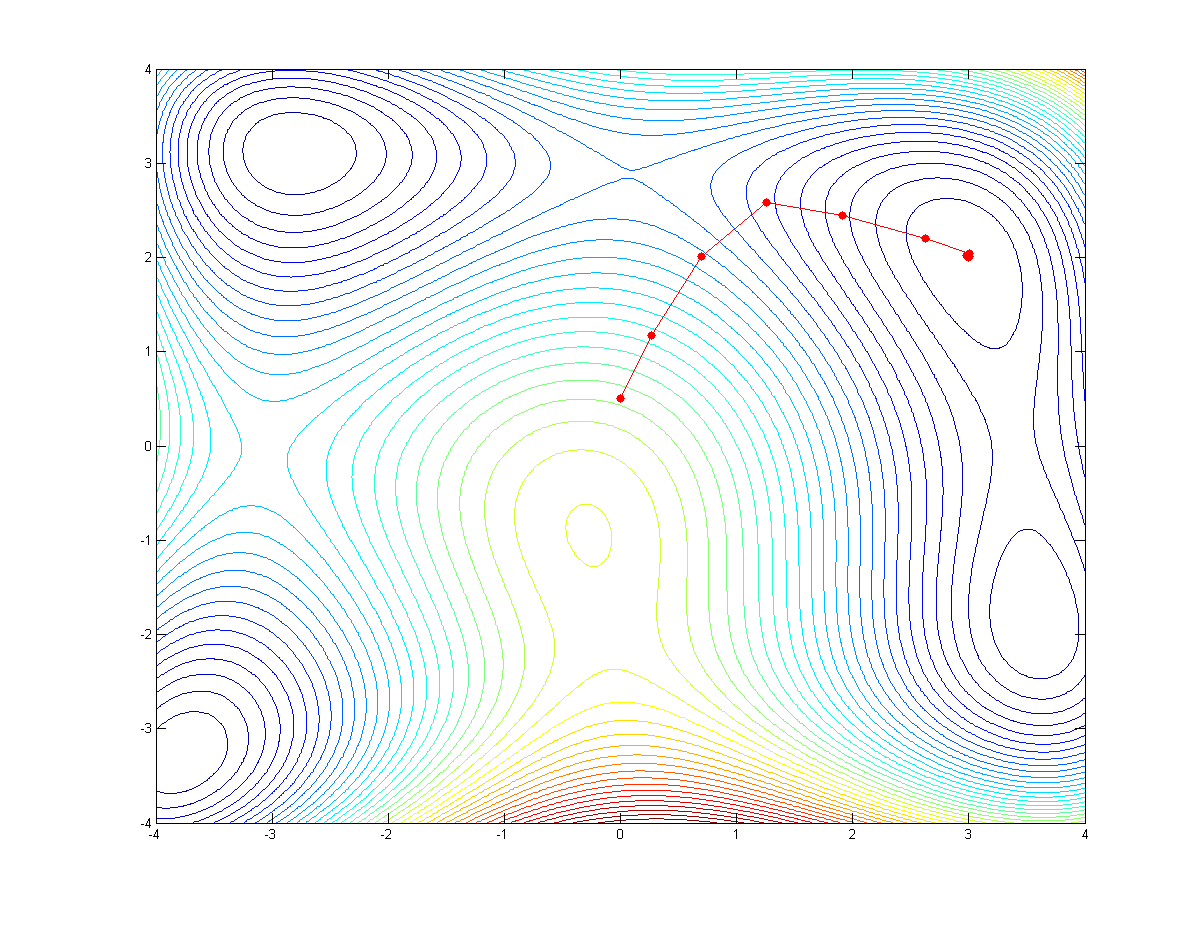
\includegraphics[width=\textwidth]{../bilder/recht_wink/const_a.png}
\caption{normales Gradientenverfahren}\label{vergleich_a}
\end{subfigure} \begin{subfigure}[b]{0.49\textwidth}
\centering
%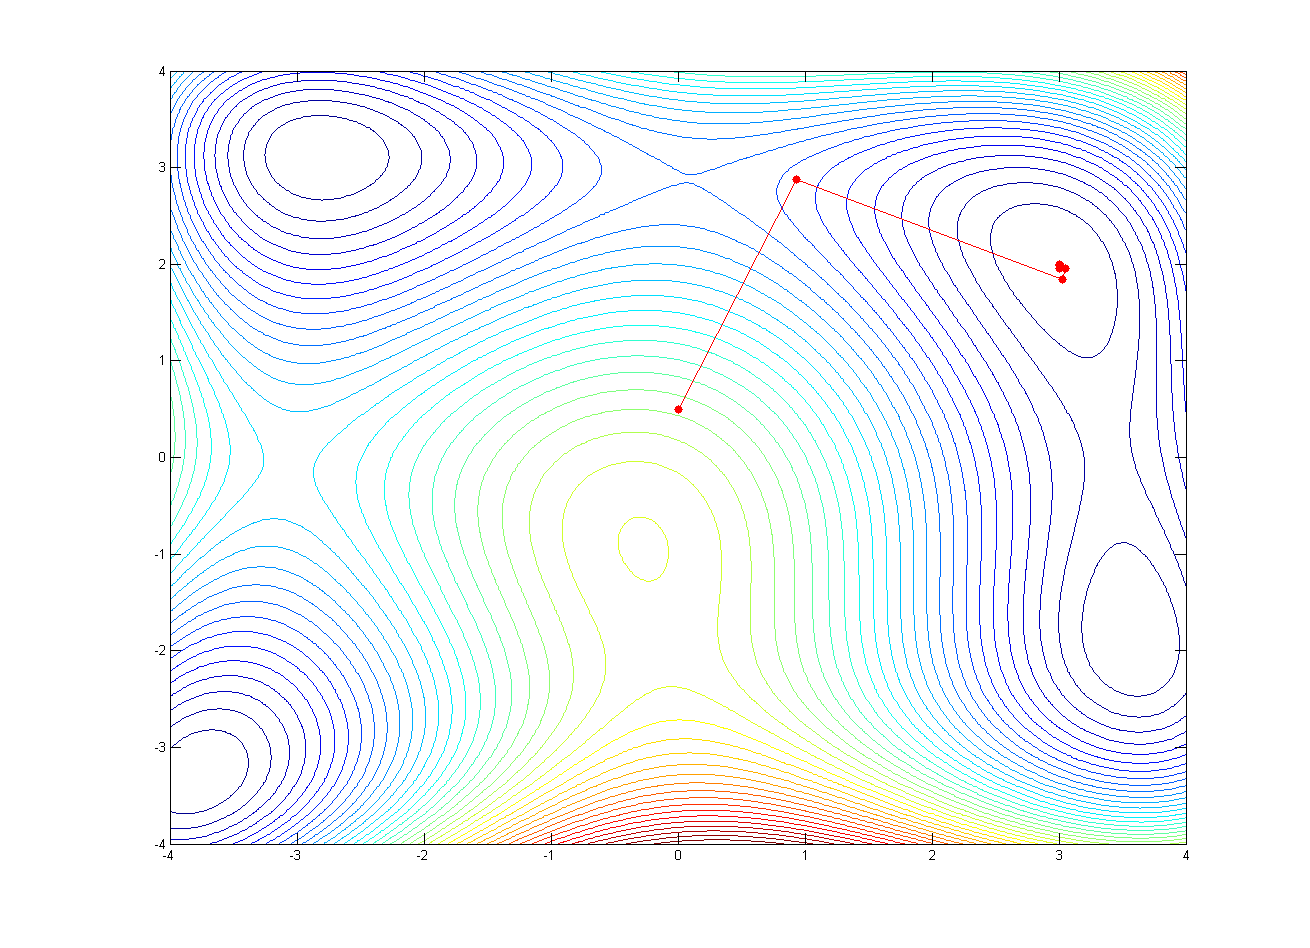
\includegraphics[width=\textwidth]{../bilder/recht_wink/rw_1.png}
\caption{mit Optimierung}\label{vergleich_b}
\end{subfigure}
\caption{Einfluss der Optimierung}
\end{figure}


\figref{vergleich_a} zeigt die Vorgehensweise auf den vorherigen
Seiten. In diesem Beispiel wurde mit konstanten Schrittweiten
gearbeitet. Durch die Auswertung der Schrittweiten konnte f"ur dieses
Problem eine optimale Weite gew"ahlt werden. So konnte eine L"osung
gefunden werden, welche lediglich 21 Iterationsschritte ben"otigt.
Mit dem optimierten Verfahren (siehe \figref{vergleich_b}) ben"otigt man
f"ur die L"osung dieses Problems zwar 22 Iterationsschritte, braucht die
Schrittweite aber nicht zu definieren, was das Verfahren praxistauglich
macht.
